\section{Interpretability}

\begin{frame}{Interpretability}
    思想:如果给模型一个输入,模型直接输出一个结果,模型对用户来说是一个黑箱,这对一些场景下是不合适的。希望模型能够输出一些直观解释,让用户能理解模型的决策过程。

    几种方法:
    \begin{itemize}
        \item LIME Algorithm
        \item Integrated Method
        \item SHAP
    \end{itemize}
\end{frame}

\begin{frame}{LIME}
    一般框架:
    \begin{itemize}
        \item 设希望被解释的模型为 $f: \mathbb{R}^{d}\to \mathbb{R}$,输入为 $x$。目标:解释为什么 $f(x)$ 这样输出。
        \item 设 $g \in G$ 是一个解释模型,定义域为 $\left\{ 0, 1 \right\}^{d'} $代表 $x$可解释的表示的二进制向量。
        \item $\Omega(g)$代表解释的复杂度度量。
        \item $\Pi_x(z)$ 表示 instance $z$ 与 $x$ 的接近程度。
        \item 目标:最小化 $\xi(x) = \text{arg}\min_{g \in G}\left( L(f, g, \Pi_x) + \Omega(g) \right) $,$\xi(x)$ 就是最优解释。
    \end{itemize}
    我们只考虑 $G$ 是线性模型族的情况,即 $g(z') = w_g \cdot z'$。
    
    通常取 $L(f, g, \Pi_x) = \sum_{z, z' \in Z} \Pi_x (z) \cdot (f(z) - g(z'))^{2}$,其中$\Pi_x(z) = \exp\left( - D(x, z)^{2} / \sigma^{2} \right) $,$\Omega(g) = \infty \mathbbm 1[\left\| w_g \right\| _0 > k]$

\end{frame}

\begin{frame}{LIME Algorithm}
    算法:
    \begin{center}
        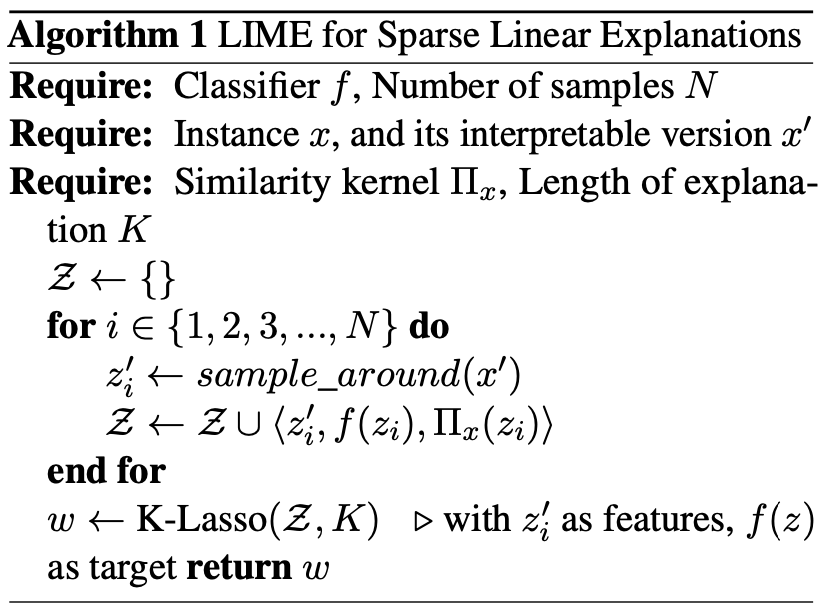
\includegraphics[width=0.6\textwidth]{assets/lime.png}
    \end{center}
\end{frame}

\begin{frame}{LIME Algorithm}
\begin{itemize}
    \item 在图像分类模型解释问题中,每个可解释的$z$是对每个super-pixel分配0或1。
    \item 为了解释为什么模型将一个弹着吉他的狗头人识别出来是Labrador、Electric guitar和Acoustic guitar,按照上述算法中$K-Lasso$ 的原理,最终每种标签对应的返回权重$w$是比较稀疏的,将这些非$0$的$w$分量对应的super-pixel按原图输出出来,$0$的$w$分量对应的super-pixel输出灰色图像,可得到下图。
\end{itemize}
\begin{center}
    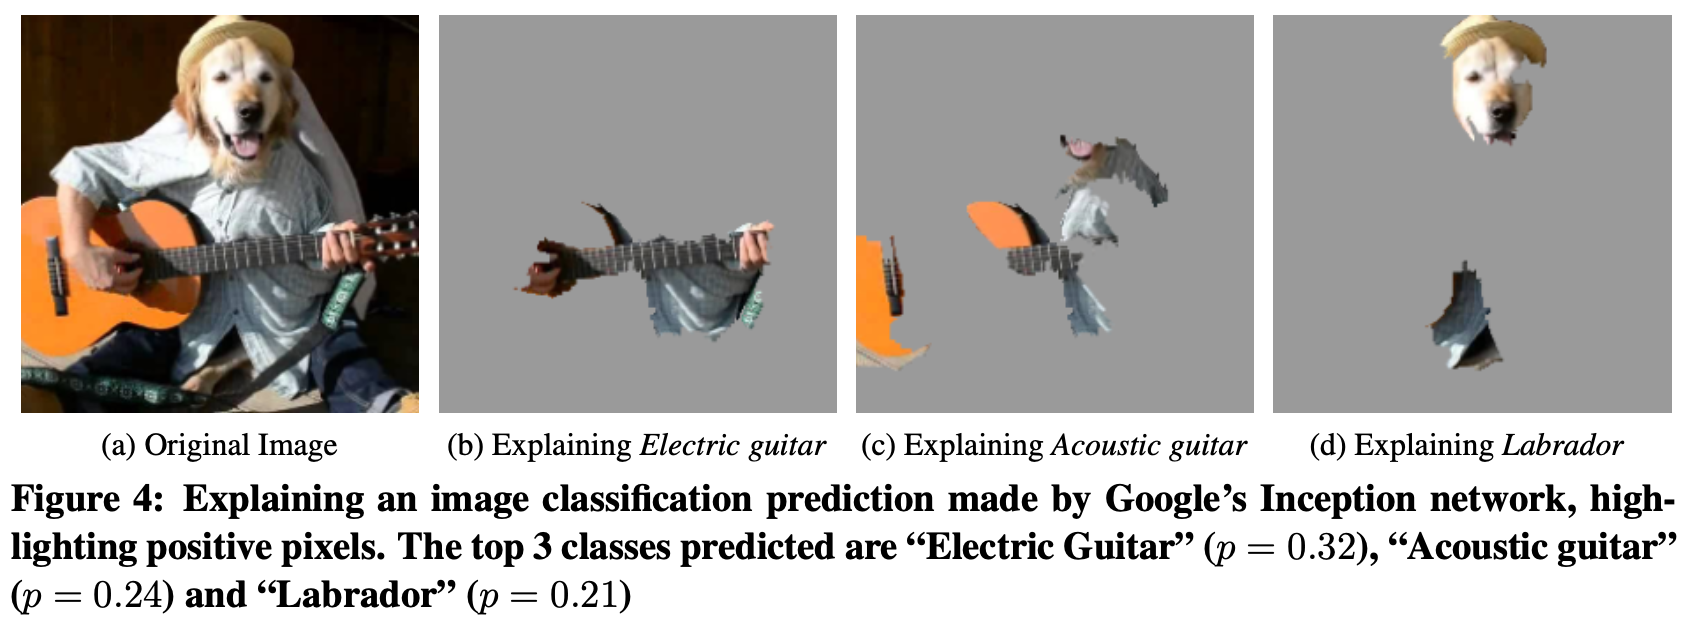
\includegraphics[width=0.75\textwidth]{assets/limee.png}
\end{center}
\end{frame}

\begin{frame}{Integrated Method}
    思想:Integrated Method论文中指出了一些关于可解释性的公理,然后从这些公理出发推导可能的解释方法。Integrated Gradients满足所有他们提出的公理。

    \begin{itemize}
        \item 设函数 $F: \mathbb{R}^{n} \to [0, 1]$ 表示一个 deep network,$x\in \mathbb{R}^{n}$ 是输入,$x'\in \mathbb{R}^{n}$ 是一个 baseline input。
        \item 定义 
        \[
        \text{IntegratedGrads}_i(x) := (x_i - x'_i) \cdot \int_{\alpha=0}^{1} \frac{\partial F(x' + \alpha(x - x'))}{\partial x_i}  \mathrm{d}\alpha  
        \]
        \item Completeness: 
        \[
        \sum_{i=1}^{n}\text{IntegratedGrads}_i(x) = F(x) - F(x')
        \]
        证明方法:简单的微积分。
    \end{itemize}
\end{frame}

\begin{frame}{Shapley Value Algorithm (a.k.a. SHAP)}
    \begin{itemize}
        \item 问题:$x_1, x_2, \cdots, x_n$ 是输入变量,$S \subseteq \left\{ x_1, x_2, \cdots, x_n \right\} $, $f(S)$ 表示 $S$ 对最终结果的贡献。如何计算每个输入变量单独的作用?
        \item 生动的例子:抢银行分钱,总钱数为 $f([n])$.
        \item $x_i$ 的作用是($x_i$应该分得的钱)
    \[
        \phi_i(f) = \sum_{S \subseteq [n]\backslash \left\{ i \right\}} \frac{\left| S \right| ! \left( n - |S| - 1 \right) !}{n!} \Big( f(S \cup \left\{ i \right\}) - f(S) \Big)
    \]
    \item 性质:
    \[
        \sum_{i=1}^{n} \phi_i(f) = f([n])  
    \]
    \end{itemize}
\end{frame}
